\section{From a cone map with a full corner to a dimension-drop map}
\label{sec:dimension-drop}

Recall the unitized matrix cone
\[
C=\{f\in C([0,1],M_2):f(0)\in\C1\},
\qquad \iota(t)=t.
\]
We show that a unital map from \(C\) whose first matrix corner is full
produces a unital dimension-drop map after taking a finite tensor power.
The comparison we construct has a fixed cutoff: the defect of an exactly
equivalent orthogonal pair is Cuntz below the positive part of its first
element minus \(1/2\). Two elementary constructions in tensor powers of
\(C\) will be useful. The first identifies these tensor powers with
matrix-valued functions on a cube; the second moves a copy of \(M_2\)
continuously between the available tensor factors.

\begin{lemma}\label{lem:cone-cube}
For \(k\ge1\), the algebra \(C^{\otimes k}\) identifies with
\[
\left\{
 f\in C([0,1]^k,M_2^{\otimes k}):
 f(t)\in\bigotimes_{i=1}^k E_i(t)
\right\},
\qquad
E_i(t)=
\begin{cases}
M_2,&t_i>0,\\
\C1,&t_i=0.
\end{cases}
\]
\end{lemma}

\begin{proof}
The algebra \(C\) is nuclear, being the unitization of
\(C_0((0,1])\otimes M_2\). Its maximal and minimal tensor powers therefore
agree. The natural map from its minimal tensor power into
\(C([0,1]^k,M_2^{\otimes k})\) is isometric: the direct sum of point
evaluations is a faithful representation of \(C\), and its spatial
tensor power is the direct sum of the evaluations on the cube.
The range satisfies the indicated boundary conditions.

To prove the reverse inclusion, choose a vector-space basis
\(b_0,b_1,b_2,b_3\) of \(M_2\) with \(b_0=1\), and write a section as
\[
f(t)=
\sum_{\alpha\in\{0,1,2,3\}^k}
f_\alpha(t)\,
b_{\alpha_1}\otimes\cdots\otimes b_{\alpha_k}.
\]
Its scalar coefficients are continuous. If
\(S_\alpha=\{i:\alpha_i\ne0\}\), the boundary conditions say that
\(f_\alpha(t)=0\) whenever \(t_i=0\) for some \(i\in S_\alpha\).
Put \(p_\alpha(t)=\prod_{i\in S_\alpha}t_i\), with empty product equal
to one. Then
\[
f_\alpha(t)\frac{p_\alpha(t)}{p_\alpha(t)+\varepsilon}
\longrightarrow f_\alpha(t)
\quad\text{uniformly as }\varepsilon\downarrow0.
\]
Indeed, \(f_\alpha\) vanishes on the zero set of \(p_\alpha\), and is
uniformly small on sufficiently small sublevel sets of \(p_\alpha\);
on their complements the displayed convergence is uniform.
Thus \(f_\alpha\) belongs to the closed scalar ideal generated by
\(p_\alpha\).

Every continuous scalar function on the cube, multiplied by the matrix
identity, lies in \(C^{\otimes k}\), by approximation by finite sums of
products of one-variable functions. Moreover,
\[
p_\alpha(t)\,
b_{\alpha_1}\otimes\cdots\otimes b_{\alpha_k}
\]
is an elementary tensor of elements of \(C\): its \(i\)-th factor is
\(\iota b_{\alpha_i}\) if \(i\in S_\alpha\), and is \(1\) otherwise.
The scalar-ideal approximation now puts each summand of \(f\), and hence
\(f\) itself, in \(C^{\otimes k}\).
\end{proof}

\begin{lemma}\label{lem:matrix-simplex}
For every \(k\ge1\), there is a point-norm continuous family of unital
\(*\)-homomorphisms
\[
\theta_r:M_2\longrightarrow M_2^{\otimes k},
\qquad
r\in\Delta_{k-1}
=\left\{r\in[0,1]^k:\sum_i r_i=1\right\},
\]
whose range uses only the tensor factors indexed by \(\{i:r_i>0\}\).
At the \(j\)-th vertex, \(\theta_r\) is the \(j\)-th coordinate inclusion.
\end{lemma}

\begin{proof}
Let \(F\in M_2\otimes M_2\) be the flip unitary, and fix the unitary path
\[
U(s)=\frac{1+F}{2}+e^{i\pi s}\frac{1-F}{2},
\qquad 0\le s\le1.
\]
Thus \(U(0)=1\), \(U(1)=F\), and
\(F(a\otimes1)F^*=1\otimes a\).

Proceed by induction on \(k\), starting with the identity map when
\(k=1\). For \(r_k<1\), let \(\tau:M_2\to M_2^{\otimes(k-1)}\) be the
map supplied by induction for
\[
\left(\frac{r_1}{1-r_k},\ldots,\frac{r_{k-1}}{1-r_k}\right),
\]
and set
\[
\theta_r(a)
=(\tau\otimes\id)
\bigl(U(r_k)(a\otimes1)U(r_k)^*\bigr).
\]
This is a unital \(*\)-homomorphism, varying continuously where
\(r_k<1\). At \(r_k=1\), define
\(\theta_r(a)=1^{\otimes(k-1)}\otimes a\). For every preceding map
\(\tau\), contractivity gives
\[
\begin{aligned}
\|\theta_r(a)-1^{\otimes(k-1)}\otimes a\|
&\le
\|U(r_k)(a\otimes1)U(r_k)^*-F(a\otimes1)F^*\|\\
&\le 2\|a\|\,\|U(r_k)-F\|.
\end{aligned}
\]
The last quantity tends to zero as \(r_k\to1\), uniformly in \(\tau\).
This proves continuity even when the normalized preceding weights
have no limit.

If \(r_k=0\), the formula is exactly \(\tau(a)\otimes1\).
If \(r_i=0\) for an earlier index, the induction hypothesis makes
the \(i\)-th tensor factor scalar throughout the range of \(\tau\),
and applying \(\tau\otimes\id\) preserves this restriction.
These observations prove the support condition on every face, as well
as the assertion at the vertices.
\end{proof}

\begin{proposition}\label{prop:cone-drop}
Let \(P\) be a nonzero unital \(C^*\)-algebra. Suppose that there is a
unital \(*\)-homomorphism \(\eta:C\to P\) such that
\(\eta(\iota e_{11})\) is full in \(P\). Then, for some finite
\(m\ge1\), the maximal tensor power \(B=P^{\otimes m}\) contains
orthogonal positive contractions \(b_1,b_2\) and an element \(v_B\)
such that
\[
b_1=v_B^*v_B,\qquad b_2=v_Bv_B^*,\qquad
1_B-b_1-b_2\precsim(b_1-1/2)_+.
\]
Consequently there is a unital \(*\)-homomorphism
\[
I(2,3)\longrightarrow P^{\otimes m}.
\]
\end{proposition}

\begin{proof}
We first obtain a finite comparison constant from fullness. An auxiliary
tensor power will provide an element whose class is both small enough to
fit that many copies under the unit and large enough to dominate the
unit after another finite amplification. The cube construction then
places the defect under elements on which the first member of the pair
acts as the identity.

\emph{A full cut and its comparison.}
Write \(b=\eta(\iota e_{11})\). By fullness, choose
\(h_i,\ell_i\in P\), \(1\le i\le N\), such that
\[
\left\|1_P-\sum_{i=1}^N h_i b\ell_i\right\|<\frac12.
\]
For sufficiently small \(0<\delta<1\), the element
\[
c=(b-\delta)_+
=\eta(q),\qquad
q(t)=(t-\delta)_+e_{11},
\]
still satisfies
\(\|1_P-S\|<1\), where \(S=\sum_i h_i c\ell_i\).
Thus \(S\) is invertible, and \(c\) is full.

We record an exact matrix comparison. Put
\[
T=(h_1c^{1/2},\ldots,h_Nc^{1/2}),\qquad
Z=(c^{1/2}\ell_1,\ldots,c^{1/2}\ell_N)^{\mathrm T},
\qquad d=Z^*Z.
\]
Since \(S=TZ\), we have
\[
S^*S\le\|T\|^2d.
\]
Invertibility of \(S\) therefore implies invertibility of \(d\).
The column \(V=(\ell_i d^{-1/2})_{i=1}^N\) satisfies
\begin{equation}\label{eq:full-cut-comparison}
V^*\operatorname{diag}(c,\ldots,c)V=1_P,
\qquad\text{so}\qquad [1_P]\le N[c].
\end{equation}

\emph{An auxiliary amplification.}
Let \(c_1=c\) and \(c_2=\eta((\iota-\delta)_+e_{22})\).
These are orthogonal equivalent positive contractions, with equivalence
witness \(\eta(\sqrt{(\iota-\delta)_+}\,e_{21})\), and
\(c_1+c_2\le1_P\).
Choose \(L\ge1\) such that \(2^L\ge N\), and set
\[
R=P^{\otimes L},\qquad e=c^{\otimes L},\qquad k=N^L.
\]
The \(2^L\) elements
\[
c_{\sigma_1}\otimes\cdots\otimes c_{\sigma_L},
\qquad \sigma\in\{1,2\}^L,
\]
are pairwise orthogonal, all have Cuntz class \([e]\), and have sum
\((c_1+c_2)^{\otimes L}\le1_R\).
Tensoring \eqref{eq:full-cut-comparison} \(L\) times gives the other
bound in
\begin{equation}\label{eq:cone-amplification}
N[e]\le2^L[e]\le[1_R]\le N^L[e]=k[e].
\end{equation}
The two integers play different roles: \(N\) is the comparison constant
from fullness, whereas \(k\) will be the number of cube coordinates.
Both are finite and may depend on \(P\) and \(\eta\).
After applying \(\eta^{\otimes k}\), the cube construction below will supply
positive elements \(X,Y\in P^{\otimes k}\) with \(k[X]\le N[Y]\).
The two bounds on \([e]\) will then combine with this
inequality to give \([X\otimes1_R]\le[Y\otimes1_R]\).

\emph{An orthogonal pair in the cube.}
We next work in the cube model of \(C^{\otimes k}\) from
Lemma~\ref{lem:cone-cube}. Regard scalar functions as scalar matrix
functions, and define
\[
g(s)=(1-2s/\delta)_+,\qquad
H(t)=1-\prod_{j=1}^k g(t_j).
\]
For \(t\ne0\), put
\[
d(t)=\max_j t_j,\qquad
r_i(t)=
\frac{(t_i/d(t)-1/2)_+}
{\sum_{j=1}^k(t_j/d(t)-1/2)_+}.
\]
At least one term in the denominator is \(1/2\), so \(r(t)\) is
well defined and continuous off the origin. Let \(\theta_r\) be the
family from Lemma~\ref{lem:matrix-simplex}, and set
\[
a_i(t)=H(t)\theta_{r(t)}(e_{ii})\quad(i=1,2),\qquad
v(t)=\sqrt{H(t)}\,\theta_{r(t)}(e_{21})
\quad(t\ne0).
\]
Set all three functions equal to zero at the origin.
The bounds
\[
0\le H(t)\le\frac{2}{\delta}\sum_j t_j,\qquad
\|a_i(t)\|\le H(t),\qquad
\|v(t)\|\le\sqrt{H(t)}
\]
prove continuity there. If \(t\ne0\) and \(t_j=0\), then \(r_j(t)=0\), so the
support condition on \(\theta\) supplies the scalar boundary condition
in that tensor factor. Consequently \(a_1,a_2,v\in C^{\otimes k}\).
They satisfy
\begin{equation}\label{eq:cone-positive-pair}
v^*v=a_1,\qquad vv^*=a_2,\qquad a_1a_2=0,\qquad
a_1+a_2=H1.
\end{equation}
In particular \(a_1,a_2\) are equivalent orthogonal positive
contractions, and their defect is
\[
X=1-a_1-a_2=g^{\otimes k}.
\]

For \(1\le j\le k\), define
\[
y_j=g^{\otimes(j-1)}\otimes q\otimes g^{\otimes(k-j)}.
\]
The \(y_j\) are positive and pairwise orthogonal, because \(qg=0\).
Moreover,
\begin{equation}\label{eq:cone-local-support}
a_1y_j=y_j\qquad(1\le j\le k).
\end{equation}
Indeed, wherever \(y_j(t)\ne0\), one has \(t_j>\delta\) and
\(t_i<\delta/2\) for every \(i\ne j\). Hence \(d(t)=t_j\) and
\(t_i/d(t)<1/2\) for all \(i\ne j\). The vector \(r(t)\) is therefore
exactly the \(j\)-th vertex, while \(H(t)=1\).
At that vertex \(\theta_{r(t)}(e_{11})\) acts as the identity on
the \(q\)-factor of \(y_j(t)\). At all other points with \(y_j(t)=0\),
the desired identity is immediate.
Figure~\ref{fig:cone-support} illustrates this localization in two
coordinates.

\begin{figure}[tbp]
\centering
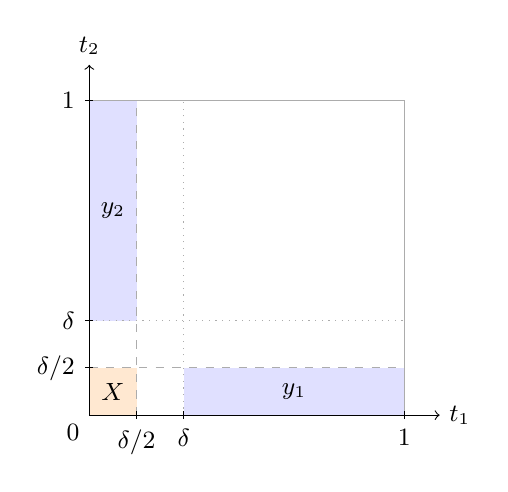
\begin{tikzpicture}[x=1cm,y=1cm,font=\small]
  \fill[orange!18] (0,0) rectangle (0.6,0.6);
  \fill[blue!12] (1.2,0) rectangle (4,0.6);
  \fill[blue!12] (0,1.2) rectangle (0.6,4);
  \draw[gray!65,thin] (0,0) rectangle (4,4);
  \draw[gray!65,dashed,thin] (0.6,0) -- (0.6,4);
  \draw[gray!65,dashed,thin] (0,0.6) -- (4,0.6);
  \draw[gray!65,dotted,thin] (1.2,0) -- (1.2,4);
  \draw[gray!65,dotted,thin] (0,1.2) -- (4,1.2);
  \draw[->] (0,0) -- (4.45,0) node[right] {$t_1$};
  \draw[->] (0,0) -- (0,4.45) node[above] {$t_2$};
  \node[below left] at (0,0) {$0$};
  \foreach \x/\ticktext in {0.6/{\delta/2},1.2/{\delta},4/{1}} {
    \draw (\x,0.05) -- (\x,-0.05);
    \node[below] at (\x,-0.06) {$\ticktext$};
    \draw (0.05,\x) -- (-0.05,\x);
    \node[left] at (-0.06,\x) {$\ticktext$};
  }
  \node at (0.3,0.3) {$X$};
  \node at (2.6,0.3) {$y_1$};
  \node at (0.3,2.6) {$y_2$};
\end{tikzpicture}

\caption{Support geometry for \(k=2\), drawn schematically. Shading
shows the closures of the regions where \(X\), \(y_1\), and \(y_2\)
can be nonzero. In the \(y_j\) region, \(r(t)\) is the \(j\)-th vertex
and \(H(t)=1\), giving \eqref{eq:cone-local-support}.}
\label{fig:cone-support}
\end{figure}

Use the same letters for the images of these elements under
\(\eta^{\otimes k}:C^{\otimes k}\to P^{\otimes k}\), and put
\(Y=\sum_{j=1}^k y_j\). All the identities just proved persist.
Writing \(G=\eta(g)\), we have
\([G]\le[1_P]\le N[c]\).
Tensor this comparison with \(G\) in the other \(k-1\) positions to
obtain
\[
[X]\le N[y_j]\quad(1\le j\le k).
\]
Adding these comparisons and using orthogonality gives
\begin{equation}\label{eq:cone-defect-sum}
k[X]\le N\sum_{j=1}^k[y_j]=N[Y].
\end{equation}
Thus the cube supplies \(k\) copies of the defect below \(N\) copies of
an element supported where \(a_1=1\). The auxiliary algebra \(R\) was
chosen precisely to remove these unequal multiplicities without any
cancellation in the Cuntz order.

\emph{Absorbing the defect.}
Finally, work in
\[
B=P^{\otimes k}\otimes R=P^{\otimes(k+L)},
\qquad b_i=a_i\otimes1_R.
\]
Since \(a_1Y=Y\), taking adjoints gives \(Ya_1=Y\).
Thus \(a_1\) and \(Y\) commute, and functional calculus gives
\((a_1-1/2)_+Y=Y/2\). In particular the element
\(z=\sqrt{2Y}\otimes1_R\) satisfies
\[
z^*(b_1-1/2)_+z=Y\otimes1_R.
\]
The following use of tensor divisibility to obtain comparison follows
the pattern of Robert and R\o rdam \cite[Lemma~6.1(i)]{RR}; we verify the
comparisons directly in maximal tensor products. Together with
\eqref{eq:cone-amplification} and
\eqref{eq:cone-defect-sum}, this yields
\[
\begin{aligned}
[X\otimes1_R]
&\le k[X\otimes e]\\
&\le N[Y\otimes e]\\
&\le[Y\otimes1_R]\\
&\le[(b_1-1/2)_+].
\end{aligned}
\]
The first comparison tensors \([1_R]\le k[e]\) with \(X\), the
second tensors \eqref{eq:cone-defect-sum} with \(e\), and the third
tensors \(N[e]\le[1_R]\) with \(Y\). The last uses the exact witness
\(z\). These are comparisons in finite matrices over the maximal
tensor product \(B\).

To express the conclusion inside \(B\) itself, recall that if
\(a,b\in B_+\) and
\[
W_n^*(b\oplus0)W_n\longrightarrow a\oplus0
\]
in finite matrices, compression to the upper-left corner gives
\((W_n)_{11}^*b(W_n)_{11}\to a\).
The final comparison therefore gives
\[
1_B-b_1-b_2=X\otimes1_R\precsim(b_1-1/2)_+
\quad\text{in }B.
\]
By \eqref{eq:cone-positive-pair}, the elements \(b_1,b_2\) are
orthogonal positive contractions with exact equivalence witness
\(v_B=v\otimes1_R\in B\). This proves the asserted pair and defect
comparison. Proposition~\ref{prop:rw}, with cutoff \(1/2\),
now gives a unital \(*\)-homomorphism \(I(2,3)\to B\).
Taking \(m=k+L\) completes the proof.
\end{proof}
